%%%%%%%%%%%%%%%%%%%%%%%%%%%%%%%%%%%%%%%%%%%%%%%%%%%%%%%%%%%%%%%%%%%%%%%%%%%%%%%%%%
\documentclass[12pt]{article}
\usepackage{graphics}
\usepackage{graphicx}    	% needed for including graphics e.g. EPS, PS
\usepackage{subfigure}
\usepackage{amsmath}

\usepackage[colorlinks, bookmarks=false]{hyperref}
\hypersetup{
    colorlinks,
    citecolor=black,
    filecolor=black,
    linkcolor=black,
    urlcolor=black
}
\topmargin -1.5cm        	% read Lamport p.163
\oddsidemargin -0.04cm   	% read Lamport p.163
\evensidemargin -0.04cm  	% same as oddsidemargin but for left-hand pages
\textwidth 16.59cm
\textheight 21.94cm 
%\pagestyle{empty}       	% Uncomment if don't want page numbers
\parskip 7.2pt           	% sets spacing between paragraphs
%\renewcommand{\baselinestretch}{1.5} % Uncomment for 1.5 spacing between lines
\parindent 0pt		 				% sets leading space for paragraphs%%%%%%%%%%%%%%%%%%%%%%%%%%%%%%%%%%%%%%%%%%%%%%%%%%%%%%%%%%%%%%%%%%%%%%%%%%%%%%%%%%

\newcommand{\degree}{\ensuremath{^\circ}}

\title{Handr\'{e}: An Experimental Approach to Intelligent Character/Word Recognition using Support Vector Machines \& Dynamic Time Warping}
\date{\today}
\author{
	Sang Woo Jun \\ 
	wjun@mit.edu \\ 
  \and
  Chong-U Lim\\
  culim@mit.edu
}

\begin{document}

\maketitle

\begin{abstract}
	Optical Character Recognition (OCR) is the term used to describe the process of recognizing scanned images of text from documents, which may be handwritten manuscripts or printed text. An extension to OCR is Intelligent Character Recognition (ICR), which involves additional processing and recognition techniques in order to improve the accuracy of translating such documents by performing recognition on the level of words as opposed to individual characters. In this paper, we present an experimental system to outline the process of performing recognition of an entire handwritten document. Our approach outlines the feasibility of performing word recognition without having to collect hand-written samples for training. We make use of a windowed time-series method and pixel analysis to perform segmentation of the document invididual words and characters respectively. To perform individual character recognition, we used 2 different approaches -- a kernel-based support vector machine (SVM) classifier and a dynamic time-warping (DTW) method which were both trained using a database of TrueType fonts. We then perform a committee based process of combining results from both models together with a probablistic spelling checker in order to perform the word recognition. 
\end{abstract}

\newpage
\tableofcontents
\newpage
\section{Introduction}

\section{Segmentation}
\label{section:segmentation}
	\subsection{Word Segmentation}
		\subsubsection{Time-series Segmentation}
		Lorem ipsum dolor sit amet, consectetur adipiscing elit. Quisque posuere molestie metus. Suspendisse tellus urna, porta sit amet rutrum eu, tristique quis urna. Donec varius pharetra purus, eget mollis tortor ornare vel. Nullam sagittis tellus id dui placerat eget congue libero facilisis. Donec mattis sagittis lectus, eget porta quam facilisis vel. Vestibulum non urna ante, nec mattis mauris. Nulla sit amet interdum eros. Nam congue lacinia nulla, vitae aliquet nisl tincidunt vel. Morbi gravida bibendum ipsum, at accumsan nisl suscipit ac. Sed accumsan cursus tortor a faucibus. Phasellus tempus, orci ac lacinia hendrerit, dui justo accumsan mi, congue dapibus massa turpis at lectus. Cras a tellus nisi. Aliquam vitae dolor id nunc lacinia fermentum et sit amet metus. Nullam viverra ante eu mauris ultrices nec adipiscing lectus dapibus. Class aptent taciti sociosqu ad litora torquent per conubia nostra, per inceptos himenaeos. Nam mollis commodo lacus, eget bibendum risus lobortis nec.
		\subsubsection{Post-processing}
		Lorem ipsum dolor sit amet, consectetur adipiscing elit. Quisque posuere molestie metus. Suspendisse tellus urna, porta sit amet rutrum eu, tristique quis urna. Donec varius pharetra purus, eget mollis tortor ornare vel. Nullam sagittis tellus id dui placerat eget congue libero facilisis. Donec mattis sagittis lectus, eget porta quam facilisis vel. Vestibulum non urna ante, nec mattis mauris. Nulla sit amet interdum eros. Nam congue lacinia nulla, vitae aliquet nisl tincidunt vel. Morbi gravida bibendum ipsum, at accumsan nisl suscipit ac. Sed accumsan cursus tortor a faucibus. Phasellus tempus, orci ac lacinia hendrerit, dui justo accumsan mi, congue dapibus massa turpis at lectus. Cras a tellus nisi. Aliquam vitae dolor id nunc lacinia fermentum et sit amet metus. Nullam viverra ante eu mauris ultrices nec adipiscing lectus dapibus. Class aptent taciti sociosqu ad litora torquent per conubia nostra, per inceptos himenaeos. Nam mollis commodo lacus, eget bibendum risus lobortis nec.

	\subsection{Character Segmentation}
		\subsubsection{Pre-processing}
		Hand-labeled Training
		Lorem ipsum dolor sit amet, consectetur adipiscing elit. Quisque posuere molestie metus. Suspendisse tellus urna, porta sit amet rutrum eu, tristique quis urna. Donec varius pharetra purus, eget mollis tortor ornare vel. Nullam sagittis tellus id dui placerat eget congue libero facilisis. Donec mattis sagittis lectus, eget porta quam facilisis vel. Vestibulum non urna ante, nec mattis mauris. Nulla sit amet interdum eros. Nam congue lacinia nulla, vitae aliquet nisl tincidunt vel. Morbi gravida bibendum ipsum, at accumsan nisl suscipit ac. Sed accumsan cursus tortor a faucibus. Phasellus tempus, orci ac lacinia hendrerit, dui justo accumsan mi, congue dapibus massa turpis at lectus. Cras a tellus nisi. Aliquam vitae dolor id nunc lacinia fermentum et sit amet metus. Nullam viverra ante eu mauris ultrices nec adipiscing lectus dapibus. Class aptent taciti sociosqu ad litora torquent per conubia nostra, per inceptos himenaeos. Nam mollis commodo lacus, eget bibendum risus lobortis nec.
		\subsubsection{Pixel Analysis}
		Pixel Analysis
		Lorem ipsum dolor sit amet, consectetur adipiscing elit. Quisque posuere molestie metus. Suspendisse tellus urna, porta sit amet rutrum eu, tristique quis urna. Donec varius pharetra purus, eget mollis tortor ornare vel. Nullam sagittis tellus id dui placerat eget congue libero facilisis. Donec mattis sagittis lectus, eget porta quam facilisis vel. Vestibulum non urna ante, nec mattis mauris. Nulla sit amet interdum eros. Nam congue lacinia nulla, vitae aliquet nisl tincidunt vel. Morbi gravida bibendum ipsum, at accumsan nisl suscipit ac. Sed accumsan cursus tortor a faucibus. Phasellus tempus, orci ac lacinia hendrerit, dui justo accumsan mi, congue dapibus massa turpis at lectus. Cras a tellus nisi. Aliquam vitae dolor id nunc lacinia fermentum et sit amet metus. Nullam viverra ante eu mauris ultrices nec adipiscing lectus dapibus. Class aptent taciti sociosqu ad litora torquent per conubia nostra, per inceptos himenaeos. Nam mollis commodo lacus, eget bibendum risus lobortis nec.

			
\section{Recognition}
\label{section:recognition}
	In this section, we outline the techniques which we focused on in order to address recoginition task of our project. In Section~\ref{subsection:svm}, we describe desribe support vector machines (SVM) and how they can be used for classification of the different alpha-numerical characer by training on a dataset in order to learn a model which generalizes well for all characters.. Section~\ref{subsection:dtw} covers dynamic time warping, and describes our approach to using it to classify alpha-numerical characters by minimising the distance of difference between the pixel-representations of the different characters. Section~\ref{subsection:spellingcheck} explains how a spelling checker is implemented in order to act as a type of regularization of the combined results from the SVM and DTW systems.

	\subsection{Classification using Support Vector Machines}	
	\label{subsection:svm}
	Support Vector Machines (SVMs) are a form of supervized learning methods which can be used for classificaiton or regression problems. In a binary classification example, we would train the SVM on a labelled dataset and if they they are linearly separable, the SVM will find a unique separation boundary in the form of a hyperplane with points falling on each side having different classifications. The separation boundary would be one in which the margin is maximised. 

	In general, not all data points will be linearly separable often as a result of overlapping class-conditional probabilities. Also, there is a chance of overfitting on the training data points which might negatively affect the generalizability of the classifier for future points. As such, we adopt the use of \textit{slack variables} which results in a `soft margin', in which we allow some data points to be incorrectly misclassified with a certain penalty with the aim of overcome overfitting. The general formulation of SVMs as constained quadratic programming problem is as follows

	\begin{equation*}
	\label{equation:svm}
	\begin{aligned}
	& \underset{\theta}{\text{minimize}}
	& & C\sum_{i=0}^n\xi_{i} + \frac{1}{2} \parallel\mathbf{\theta}\parallel^{2}  \\
	& \text{subject to}
	& & y_{i}(\theta\cdot\mathbf{x}_{n}+\theta_{0}) \ge 1 - \xi_{i}, \; i = 1, \ldots, m
	\end{aligned}
	\end{equation*}

	where $x_{i}$ represents each training data point, with $y_{i}$ being its corresponding target classification. $\mathbf{\theta}$ is the model, or parameter, of the classifier with offset $\theta_{0}$, while C and $\xi$ represent the penalty and slack variables respectively.
	
	\subsubsection{Supporting Multiple Classes}
	In our project, we are interested in the use of SVMs to classify individual characters based the a given vector input of pixel values. Extending SVMs to support multiple target classifications requires us to train multiple binary classifiers, one for each individual target character. Given an input vector, each classifier would give a possible classification, and we then employ \textbf{voting} as a way of deciding the best classification result for our data. The common voting strategies to decide on a classification described as follows.

	\paragraph{One-versus-one}
	In one-versus-one voting, the idea is to fit a classifier for each pair of classes, and when it comes to making the prediction, we select the class with the most number of votes. 
		
	\paragraph{One-versus-rest}
	In one-versus-rest voting, each character has a classifier which is fit to it. When making the predicition, the class with the highest classification output is chosen in a \textit{winner-takes-all} strategy.

	\subsection{K-means Clustering using Dynamic Time-Warping}
	\label{subsection:dtw}
	Lorem ipsum dolor sit amet, consectetur adipiscing elit. Quisque posuere molestie metus. Suspendisse tellus urna, porta sit amet rutrum eu, tristique quis urna. Donec varius pharetra purus, eget mollis tortor ornare vel. Nullam sagittis tellus id dui placerat eget congue libero facilisis. Donec mattis sagittis lectus, eget porta quam facilisis vel. Vestibulum non urna ante, nec mattis mauris. Nulla sit amet interdum eros. Nam congue lacinia nulla, vitae aliquet nisl tincidunt vel. Morbi gravida bibendum ipsum, at accumsan nisl suscipit ac. Sed accumsan cursus tortor a faucibus. Phasellus tempus, orci ac lacinia hendrerit, dui justo accumsan mi, congue dapibus massa turpis at lectus. Cras a tellus nisi. Aliquam vitae dolor id nunc lacinia fermentum et sit amet metus. Nullam viverra ante eu mauris ultrices nec adipiscing lectus dapibus. Class aptent taciti sociosqu ad litora torquent per conubia nostra, per inceptos himenaeos. Nam mollis commodo lacus, eget bibendum risus lobortis nec.

	\subsection{Spelling Corrector}
	\label{subsection:spellingcheck}
	Lorem ipsum dolor sit amet, consectetur adipiscing elit. Quisque posuere molestie metus. Suspendisse tellus urna, porta sit amet rutrum eu, tristique quis urna. Donec varius pharetra purus, eget mollis tortor ornare vel. Nullam sagittis tellus id dui placerat eget congue libero facilisis. Donec mattis sagittis lectus, eget porta quam facilisis vel. Vestibulum non urna ante, nec mattis mauris. Nulla sit amet interdum eros. Nam congue lacinia nulla, vitae aliquet nisl tincidunt vel. Morbi gravida bibendum ipsum, at accumsan nisl suscipit ac. Sed accumsan cursus tortor a faucibus. Phasellus tempus, orci ac lacinia hendrerit, dui justo accumsan mi, congue dapibus massa turpis at lectus. Cras a tellus nisi. Aliquam vitae dolor id nunc lacinia fermentum et sit amet metus. Nullam viverra ante eu mauris ultrices nec adipiscing lectus dapibus. Class aptent taciti sociosqu ad litora torquent per conubia nostra, per inceptos himenaeos. Nam mollis commodo lacus, eget bibendum risus lobortis nec.
	
	
\section{Experimental Design}
\label{section:experiments}
In this section, we desribe the experimental design which we undertook in order to apply the segmentation and recognition techniques from Sections~\ref{section:segmentation} and~\ref{section:recognition}. In Section~\ref{subsection:experiments:svm}, we describe the prodedure in which we trained the multi-class SVMs on training data which consisted of different images of each alphabet character for a variety of fonts. Section~\ref{subsection:experiments:dtw} outlines the application of DTW onto a single font set and how it was used to perform its classification. How the results from both experiments were combined together to make committee-based decision is covered in Section~\ref{subsection:experiments:combinedchar}. Finally, Section~\ref{subsection:experiments:combinedword} explains the use of the dictionary spelling checker to improve the result and come up with a final decision.
	
	\subsection{Recognizing Alphabet Characters using Multi-Class SVMs}
	\label{subsection:experiments:svm}
	For the purpose of our project, we tried to locate a resource of training data for alphabets which was commonly available. Several repositories containing data were either unsuitable or was paid-only. More importantly, we wanted to show-case that system could make use of a generic database for its training data, and not have to resort in having a particular target domain to have to first provide us with both a vast number of examples, but also go through the tedious task of hand-labelling them though it given the resources and time, it might be a possible way to improve the system (Section~\ref{section:conclusion}). As such, we decided to using readily available TrueType fonts as our training data.
			
		\subsubsection{Using Font Images as Training Sets}
		We made use of fonts for our training data by randomly picking a set of handwritten fonts which are freely available on the web (see Appendix~\ref{appendix:data:font} for the list and samples.) In order to normalize the characters, we resized each character to fit as a 28x28 white-on-black square image\footnote{We referenced the dimensions used by the MNIST database, and serves as a reference point for common handwritten character sizes.}. The character is then set to black-and-white mode, in which the pixel values are either 0 (black) or 255 (white). For each character in the font, we also created additional samples of the character image by rotating the characters by an angle between [-16\degree, +16\degree]. Thus, each training sample can be viewed as a 1x784 vector of pixel values. 	
		
		\subsubsection{Training Parameters}
		In order to be train the best classifier for our recognition task, we varied the parameters and kernels used and performed cross-validation in order to select the best performing one. The following list describes the various parameters and choices we used. We optimised the parameters based on the precision score and recall score. Section~\ref{subsubsection:analysis:svm} shows the results of this experiment and the final values which we made use of.

		\begin{itemize}
			\item Radial Basis Kernel
			\begin{itemize}
				\item C = [1, 10, 100, 1000]
				\item $\gamma$ = [0.01, 0.001, 0.0001]
			\end{itemize}
			\item Linear Kernel
			\begin{itemize}
				\item C = [1, 10, 100, 1000]
			\end{itemize}
		\end{itemize}

		Additionally, we made use of both the 1-versus-1 strategy and 1-versus-rest voting schemes to perform the multi-class classification.

		\subsubsection{Testing on Handwritten Text}
		
		\begin{figure}[htbp!]
		\centering
		
\includegraphics[width=0.5\textwidth]{multivariate_test.eps}
		\label{figure:multivariate_test}
		\caption{Segmenting and normalizing a scanned image into its individual characters}
		\end{figure}
		
		Image segments containing words which were obtained from the word-segmentation step (Section~\ref{section:segmentation}) were used for tests. The images were then cleaned and individual characters were extracted for the recognition process. We perform similar normalization steps in order to make the test images have the same dimensions and format as our training data -- images have their colors inverted, are cropped and resized to 28x28 pixels. Using our optimal performing classifier, we then attempt to classify each individual character in the word of $l$ characters. An example of a test image is shown in Figure~\ref{figure:multivariate_test}

We also obtain the probability scores of each class (signifying how confident we are of our classification) to obtain a table containing $l$ rows, and each row contains a vector of 52 probabilities -- one each for the alphabets (26 upper-case and 26 lower-case characters.) As covered later in Section~\ref{subsection:experiments:combinedchar}, we will make use of this probability table to make a combined decision, together with the DTW method, in order to improve our word recognition results.
	
	\subsection{K-means Clustering using DTW}
	\label{subsection:experiments:dtw}
	Lorem ipsum dolor sit amet, consectetur adipiscing elit. Quisque posuere molestie metus. Suspendisse tellus urna, porta sit amet rutrum eu, tristique quis urna. Donec varius pharetra purus, eget mollis tortor ornare vel. Nullam sagittis tellus id dui placerat eget congue libero facilisis. Donec mattis sagittis lectus, eget porta quam facilisis vel. Vestibulum non urna ante, nec mattis mauris. Nulla sit amet interdum eros. Nam congue lacinia nulla, vitae aliquet nisl tincidunt vel. Morbi gravida bibendum ipsum, at accumsan nisl suscipit ac. Sed accumsan cursus tortor a faucibus. Phasellus tempus, orci ac lacinia hendrerit, dui justo accumsan mi, congue dapibus massa turpis at lectus. Cras a tellus nisi. Aliquam vitae dolor id nunc lacinia fermentum et sit amet metus. Nullam viverra ante eu mauris ultrices nec adipiscing lectus dapibus. Class aptent taciti sociosqu ad litora torquent per conubia nostra, per inceptos himenaeos. Nam mollis commodo lacus, eget bibendum risus lobortis nec.
	
	\subsection{Combined Character recognition}
	\label{subsection:experiments:combinedchar}
		
	With the resulting probability tables from the trained SVMs (Section~\ref{subsection:experiments:svm}) and the DTWs (Section~\ref{subsection:experiments:dtw}), we then developed a policy to select the resulting individual characters. First, each row in the probability was ordered from high to low -- with the most likely prediction in the front. Next, each character to be classified in the target string, we selected a subset from both the tables as a combined prediction by taking the intersection of the two sets. In the event that no characters are common between the two sets, we picked the most likely members from each set. 
	
	\begin{figure}[htbp!]
	\centering
	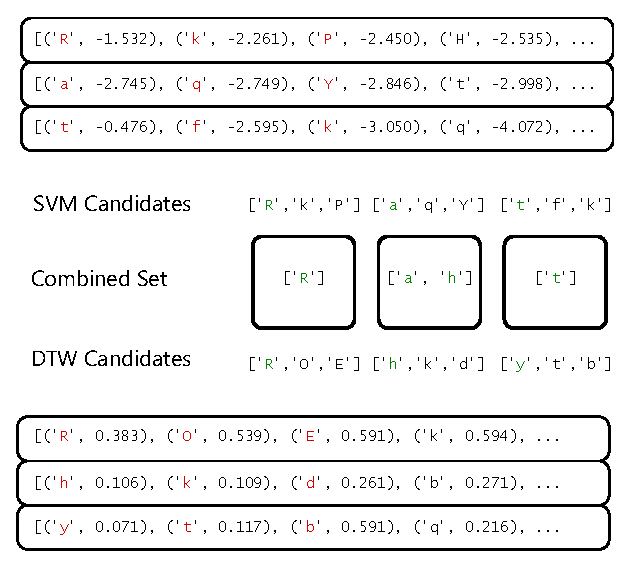
\includegraphics[width=0.5\textwidth]{combined_predictions.eps}
	\label{figure:combining_characters}
	\caption{Illustrating how predictions from both systems are combined.}
	\end{figure}
	
	
	This is illustrated in Figure~\ref{figure:combining_characters}. In this example, the scanned image contains the word `Rat'. The prediction table for the SVM system is shown at the top, while the table for the DTW system is at the bottom. For each character to be guessed, a subset of the top 3 predicted characters are chosen from both tables, so for the first character, we have the set $['R', 'k', 'p']$ and $['R', 'O', 'E']$ from the SVM system and DTW system respectively. Then, the intersection of the subets are assigned for first character of `Rat', which is `R'. For the second character, as there are no intersecting characters, we pick the top two predictions to form the subset $['a', 'h']$. The third character `t' follows the same discussion as the first character `R'.
	
	After some experimentation, we emperically decided that selecting subset of 3 characters from each prediction table row was the best policy due to potentially large number of permutations that might result from taking more. In the case where the intersecting set is empty, we picked the top predicted character from each of the tables.
	
\subsection{Combined Word recognition}
	\label{subsection:experiments:combinedword}
	Lorem ipsum dolor sit amet, consectetur adipiscing elit. Quisque posuere molestie metus. Suspendisse tellus urna, porta sit amet rutrum eu, tristique quis urna. Donec varius pharetra purus, eget mollis tortor ornare vel. Nullam sagittis tellus id dui placerat eget congue libero facilisis. Donec mattis sagittis lectus, eget porta quam facilisis vel. Vestibulum non urna ante, nec mattis mauris. Nulla sit amet interdum eros. Nam congue lacinia nulla, vitae aliquet nisl tincidunt vel. Morbi gravida bibendum ipsum, at accumsan nisl suscipit ac. Sed accumsan cursus tortor a faucibus. Phasellus tempus, orci ac lacinia hendrerit, dui justo accumsan mi, congue dapibus massa turpis at lectus. Cras a tellus nisi. Aliquam vitae dolor id nunc lacinia fermentum et sit amet metus. Nullam viverra ante eu mauris ultrices nec adipiscing lectus dapibus. Class aptent taciti sociosqu ad litora torquent per conubia nostra, per inceptos himenaeos. Nam mollis commodo lacus, eget bibendum risus lobortis nec.

\section{Results \& Analysis}
\label{section:results}
	In this section, we provide the results from the experiments conducted for the project which were explained in Section~\ref{section:experiments}. 
	
	\subsection{Alphabet Character Recognition using SVMs}
	\label{subsubsection:analysis:svm}
	
		\subsubsection{Optimal Tuning Parameters}
		\label{subsubsection:analysis:svm:params}
	
	\subsection{K-means Clustering using DTW}
	Lorem ipsum dolor sit amet, consectetur adipiscing elit. Quisque posuere molestie metus. Suspendisse tellus urna, porta sit amet rutrum eu, tristique quis urna. Donec varius pharetra purus, eget mollis tortor ornare vel. Nullam sagittis tellus id dui placerat eget congue libero facilisis. Donec mattis sagittis lectus, eget porta quam facilisis vel. Vestibulum non urna ante, nec mattis mauris. Nulla sit amet interdum eros. Nam congue lacinia nulla, vitae aliquet nisl tincidunt vel. Morbi gravida bibendum ipsum, at accumsan nisl suscipit ac. Sed accumsan cursus tortor a faucibus. Phasellus tempus, orci ac lacinia hendrerit, dui justo accumsan mi, congue dapibus massa turpis at lectus. Cras a tellus nisi. Aliquam vitae dolor id nunc lacinia fermentum et sit amet metus. Nullam viverra ante eu mauris ultrices nec adipiscing lectus dapibus. Class aptent taciti sociosqu ad litora torquent per conubia nostra, per inceptos himenaeos. Nam mollis commodo lacus, eget bibendum risus lobortis nec.
	
	\subsection{Combined Character recognition}
	Lorem ipsum dolor sit amet, consectetur adipiscing elit. Quisque posuere molestie metus. Suspendisse tellus urna, porta sit amet rutrum eu, tristique quis urna. Donec varius pharetra purus, eget mollis tortor ornare vel. Nullam sagittis tellus id dui placerat eget congue libero facilisis. Donec mattis sagittis lectus, eget porta quam facilisis vel. Vestibulum non urna ante, nec mattis mauris. Nulla sit amet interdum eros. Nam congue lacinia nulla, vitae aliquet nisl tincidunt vel. Morbi gravida bibendum ipsum, at accumsan nisl suscipit ac. Sed accumsan cursus tortor a faucibus. Phasellus tempus, orci ac lacinia hendrerit, dui justo accumsan mi, congue dapibus massa turpis at lectus. Cras a tellus nisi. Aliquam vitae dolor id nunc lacinia fermentum et sit amet metus. Nullam viverra ante eu mauris ultrices nec adipiscing lectus dapibus. Class aptent taciti sociosqu ad litora torquent per conubia nostra, per inceptos himenaeos. Nam mollis commodo lacus, eget bibendum risus lobortis nec.
	
	\subsection{Combined Word recognition}
	Lorem ipsum dolor sit amet, consectetur adipiscing elit. Quisque posuere molestie metus. Suspendisse tellus urna, porta sit amet rutrum eu, tristique quis urna. Donec varius pharetra purus, eget mollis tortor ornare vel. Nullam sagittis tellus id dui placerat eget congue libero facilisis. Donec mattis sagittis lectus, eget porta quam facilisis vel. Vestibulum non urna ante, nec mattis mauris. Nulla sit amet interdum eros. Nam congue lacinia nulla, vitae aliquet nisl tincidunt vel. Morbi gravida bibendum ipsum, at accumsan nisl suscipit ac. Sed accumsan cursus tortor a faucibus. Phasellus tempus, orci ac lacinia hendrerit, dui justo accumsan mi, congue dapibus massa turpis at lectus. Cras a tellus nisi. Aliquam vitae dolor id nunc lacinia fermentum et sit amet metus. Nullam viverra ante eu mauris ultrices nec adipiscing lectus dapibus. Class aptent taciti sociosqu ad litora torquent per conubia nostra, per inceptos himenaeos. Nam mollis commodo lacus, eget bibendum risus lobortis nec.
	
\section{Conclusions \& Future Work}
\label{section:conclusion}
	\subsection{Conclusions}
	Lorem ipsum dolor sit amet, consectetur adipiscing elit. Quisque posuere molestie metus. Suspendisse tellus urna, porta sit amet rutrum eu, tristique quis urna. Donec varius pharetra purus, eget mollis tortor ornare vel. Nullam sagittis tellus id dui placerat eget congue libero facilisis. Donec mattis sagittis lectus, eget porta quam facilisis vel. Vestibulum non urna ante, nec mattis mauris. Nulla sit amet interdum eros. Nam congue lacinia nulla, vitae aliquet nisl tincidunt vel. Morbi gravida bibendum ipsum, at accumsan nisl suscipit ac. Sed accumsan cursus tortor a faucibus. Phasellus tempus, orci ac lacinia hendrerit, dui justo accumsan mi, congue dapibus massa turpis at lectus. Cras a tellus nisi. Aliquam vitae dolor id nunc lacinia fermentum et sit amet metus. Nullam viverra ante eu mauris ultrices nec adipiscing lectus dapibus. Class aptent taciti sociosqu ad litora torquent per conubia nostra, per inceptos himenaeos. Nam mollis commodo lacus, eget bibendum risus lobortis nec.
	\subsection{Future Work}
	Lorem ipsum dolor sit amet, consectetur adipiscing elit. Quisque posuere molestie metus. Suspendisse tellus urna, porta sit amet rutrum eu, tristique quis urna. Donec varius pharetra purus, eget mollis tortor ornare vel. Nullam sagittis tellus id dui placerat eget congue libero facilisis. Donec mattis sagittis lectus, eget porta quam facilisis vel. Vestibulum non urna ante, nec mattis mauris. Nulla sit amet interdum eros. Nam congue lacinia nulla, vitae aliquet nisl tincidunt vel. Morbi gravida bibendum ipsum, at accumsan nisl suscipit ac. Sed accumsan cursus tortor a faucibus. Phasellus tempus, orci ac lacinia hendrerit, dui justo accumsan mi, congue dapibus massa turpis at lectus. Cras a tellus nisi. Aliquam vitae dolor id nunc lacinia fermentum et sit amet metus. Nullam viverra ante eu mauris ultrices nec adipiscing lectus dapibus. Class aptent taciti sociosqu ad litora torquent per conubia nostra, per inceptos himenaeos. Nam mollis commodo lacus, eget bibendum risus lobortis nec.

\section{Acknowledgements}
	We would like to thank Dahua Lin for reviewing our initial project proposal, and subsequently taking time out of his busy schedule to meet with us and provide guidance, ideas and tips on approaches tp the project. Also, we thank Prof. Leslie Kaelbling for imparting her wisdom and stimulating our ethusiasm in the topics of machine learning. 
	 
\appendix
	\section{Data \& Results}
		\subsection{Font Samples}
		\label{appendix:data:font}
	\section{Project Timeline}
		\subsection*{Week 1: 10/28 -- 11/5 }
			\begin{itemize}
				\item{Submit project proposal}
				\item{Narrow down choices to one for the project}
				\item{Read up on related papers/books}
			\end{itemize}
		\subsection*{Week 2: 11/6 -- 11/12  }
			\begin{itemize}
				\item{Continue reading related works}
				\item{Word Segmentation investigation}
				\item{Numerical digit classification investigation}
			\end{itemize}
		\subsection*{Week 3: 11/13 -- 11/19}
			\begin{itemize}
				\item{Character segmentation}
				\item{Dynamic time-warping experiments}
				\item{Alphabet characters classification investigation}
			\end{itemize}
		\subsection*{Week 4: 11/20 -- 11/26}
			\begin{itemize}
				\item{Font database}
				\item{Dynamic time-warping for classification}
				\item{SVMs for training on fonts and classification}
			\end{itemize}
		\subsection*{Week 5: 11/27 -- 12/5}
			\begin{itemize}
				\item{Improving individual results}
				\item{Heuristics for combining both predictors}
				\item{Dictionary spell-correction}
				\item{Report writing}
			\end{itemize}

	\section{Division of Labor}
	
\bibliography{air-presentation}	
\bibliographystyle{unsrt}

\end{document}

%%%%%%%%%%%%%%%%%%%%%%%%%%%%%%%%%%%%%%%%%%%%%%%%%%%%%%%%%%%%%%%%%%%%%%%%%%%%%%%%%%
